\section{Durchführung}
\label{sec:Durchführung}
\subsection{Messgeräte}
\subsubsection{Szintillator}
Die Messung wird mit Hilfe von einem Szintillatosdetektor durchgeführt. Dieser macht sich den Effekt der Lumineszenz zu nutzte. 
Lumineszenz ist die Emission von Licht mit einem charakteristischen Spektrum. Diese wird durch die Absorption von ionisierter Strahlung erzeugt. 
Dabei wird zwischen zwei Arten von Szintillatoren unterschieden. Es gibt den organischen und anorganischen Szintillator.
In diesem Versuch wird ein organischer Szintillator benutzt.  
Bei diesen wird durch Hilfe der hinzugefügten Energie der einfallenden Strahlung die Atome in einen angeregten Zustand gehoben. 
Wenn das Atom wieder in seinen normalen Zustand zurück geht, wird Energie in Form von Photonen abgegeben.

\subsubsection{Photonenvervielfacher}
Die Abgegebenen Photonen werden mit Hilfe eines Photonenvervielfacher (PMT) in einen elektrischen Impuls umgewandelt. 
Dieser besteht aus einer Photokathode, einen Verstärkersystem, das aus mehreren Dynoden besteht und einer Anode. 
Das Licht, welches durch den Szintillator entstanden ist, trifft durch das PMT-Fenster auf die Photokathode. 
Dort werden durch den Photoeffekt Elektronen emittiert. Diese werden durch ein Elektrisches Feld auf die erste Dynode fokussiert. 
Beim Auftreffen auf die Dynoden wird ein Elektron durch die Emission von Sekundärelektronen vervielfacht. Diese werden darauf auf eine nächste Dynode beschleunigt. 
Nach mehreren Dynoden, wo diese wieder vervielfacht werden, treffen die Elektronen auf eine Anode.

\noindent So wird ein Lichtblitz in einen elektrischen Impuls umgewandelt. 

\subsubsection{Zeit-Amplituden-Konverter (TAC)}
Der TAC gibt einen Spannungsimpuls ab, dessen Amplitude proportional zu der Zeit zwischen zwei einlaufenden Impulsen ist. 

%\begin{figure}
%    \centering
%    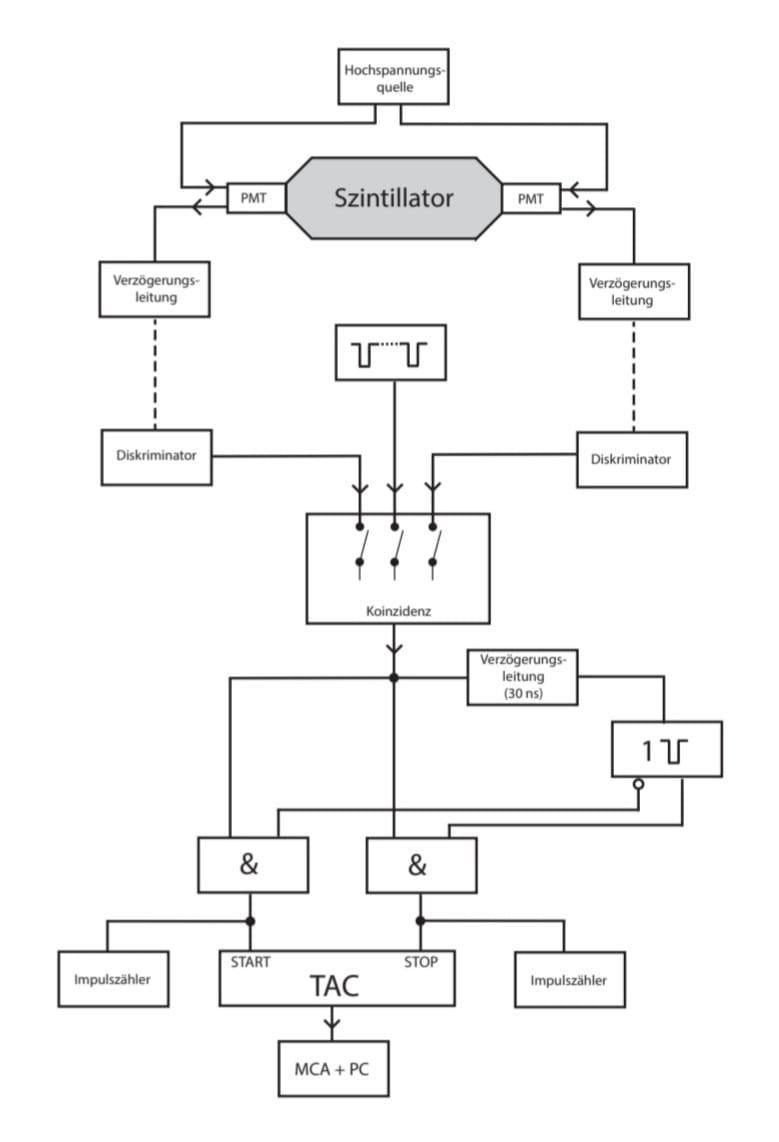
\includegraphics[width=0.8 \textwidth]{Aufbaumyon.png}
%    \caption{Aufbau %\cite{VB}.}
%    \label{fig:Auf}
%\end{figure}


\subsection{Aufbau}
Der Aufbau des Versuchs ist in Abbildung 1 dargestellt.  An den organischen Szintillator im zylinderförmigen Edelstahltank befinden sich zwei PMT angeschlossen. 
Diese geben beim der Messung eines Myons einen Impuls ab. Dieser durchläuft ein Schaltsystem bis es in einen Zeit-Amplituden-Konverter (TAC) gemessen wird.  
Dieses Signal wird dann an einen Vielkanalanalysator weitergeleitet. Der Vielkanalanalysator sortiert die einkommenden Impulse und histogrammiert diese.
Die Daten werden dann an einen Computer geleitet und gespeichert.

Da es unterschiedliche Störprozesse gibt werden unterschiedliche Bauelemente eingebaut, um diese zu unterdrücken.
Zum einen wird auch durch andere einfallende Teilchen ein Impuls ausgelöst oder auch durch eine spontane Elektronenemission der Photokathode. 
Diese Signale werden durch einen Diskriminator herausgefiltert. Nach dem Diskriminator werden die Signale von den beiden PMT im Koinzidenz zusammengeführt. 
Dieser gibt nur ein Signal weiter, wenn von beiden PMT die Signale gleichzeitig ankommen. Danach wird eine logische Schaltung durchlaufen.


\subsubsection{Logische Schaltung}
Da viele Myonen nicht im Szintillator zerfallen, werden viele Signale ausgelöst, die nicht gezählt werden sollen. Die Schaltung soll die Zeit zwischen zwei Signalen
messen, die die Lebensdauer des Myons darstellt. 
Dabei starten der erste Impuls die Zeitmessung des TACs und das zweite endet diese. 
Nun darf nur ein Impuls die Zeit stoppen, welcher beim Myonenzerfall entstanden ist und nicht eins, das durch ein anderes Myon entstanden ist, welches danach in 
den Szintillator gefallen ist. 
Daher muss nach einer gewissen Zeit, der Suchzeit, die Messung abgebrochen werden und mit einem neuen Impuls gestartet werden.
Dazu wird eine monostabile Kippstufe und zwei AND-Gatter verbaut. 
Das Startsignal stammt aus dem einem AND-Gatter, welches das Signal aus der negierten Kippstufe und die Koinzidenz vergleicht.  
Von der Koinzidenz führt dasselbe Signal über eine 30 ns Verzögerungsleitung zur Kippstufe und zu einem zweiten AND-Gatter. 
Das zweite Signal fürs AND-Gatter stammt von der Kippstufe.  Das Signal aus diesem AND-Gatter ist für den Stopimpuls zuständig.

Wenn der erste Impuls aus einer Koinzidenz kommt, wird der TAC gestartet, da die beiden Signale, die das erste AND-Gatter erreichen True sind.  
Nach 30ns kippt die Kippstufe und ein weiteres Signal stoppt die Messung. Der Zeitraum in dem die Kippstufe gekippt bleibt entspricht der Suchzeit. 
Wenn diese Zeit verstrichen ist stoppt ein weitere Impuls den TAC nicht sondern startet die Messung neu.
Um die Anzahl an Start- und Stoppimpulsen zumessen wird jeweils noch ein Impulszähler eingebaut.

\section{Durchführung}
Der Aufbau wird wie bei Abbildung 1 aufgebaut und justiert. Dabei werden zwischen den Diskriminator und den Koinzidenz Verzögerungsleitungen 
geschaltet. Diese werden so eingestellt, dass die beiden Impulse, die von einem Myon ausgelöst werden, 
gleichzeitig die Koinzidenz erreichen. Außerdem wird die Diskriminatorschwelle so eingestellt, dass bei beiden Messkanälen 
die Impulsrate ungefähr gleich ist. 
Zum Schluss wird der Vielkanalanalysator kalibriert. 
Dann wird die eigentliche Messung gestartet. Diese wird ungefähr 48 Stunden durchgeführt.

